\input{preamble}
\usepackage{tikz}
\usetikzlibrary{shapes,arrows}
\usetikzlibrary{decorations.pathreplacing}

\title{Ordinary Least Squares (Linear) Regression}

\date[]{February 17, 2015}

\begin{document}

\frame{\titlepage}

\frame{\tableofcontents}
% OLS
% Interpretation of coefficients
% Goodness-of-fit measures
% Standard errors, t-tests, p-values, and confidence intervals


\section{OLS}
\frame{\tableofcontents[currentsection]}

\frame{
	\frametitle{Uses of Regression}
	\begin{enumerate}\itemsep2em
	\item Description
	\item Prediction
	\item Causal Inference
	\end{enumerate}
}

\frame{
	\frametitle{Descriptive Inference}
	\begin{enumerate}
	\item We want to understand a \textit{population} of cases
	\item We cannot observe them all, so:
		\begin{enumerate}
    		\item Draw a \textit{representative} sample
    		\item Perform mathematical procedures on sample data
    		\item Use assumptions to make inferences about population
    		\item Express uncertainty about those inferences based on assumptions
		\end{enumerate}
	\end{enumerate}
}

\frame{
	\frametitle{Parameter Estimation}
	\begin{itemize}\itemsep1em
    	\item We want to observe population \textit{parameter} $\theta$
    	\item If we obtain a representative sample of population units:
    		\begin{itemize}
        		\item Our sample statistic $\hat{\theta}$ is an unbiased estimate of $\theta$
        		\item Our sampling procedure dictates how uncertain we are about the value of $\theta$
    		\end{itemize}
	\end{itemize}
}

\frame{
	\frametitle{Sample Estimate of Population Mean}
	We want to know $Y$ (population mean)\\
	Our \textit{estimator} is the sample mean formula which produces the sample \textit{estimate} $\bar{y}$:
	\begin{equation}
	\bar{y} = \frac{1}{n}\sum_{i=1}^{n}y_i
	\end{equation}
	where $y_i = $ value for a unit, and\\
	$n = $ sample size
	
	\begin{equation}
	SE_{\bar{y}} = \sqrt{(1-f)\frac{s^2}{n}}
	\end{equation}
	where $f = $ proportion of population sampled,\\
	$s^2 = $ sample element variance, and\\
	$n = $ sample size
}

\frame{
	\frametitle{Uncertainty}
	\begin{itemize}\itemsep1em
		\item We never know $\theta$
		\item $\hat{\theta}$ is an estimate that may not equal $\theta$
			\begin{itemize}
    			\item Unbiased due to \textbf{Law of Large Numbers}
    			\item For $\bar{y}$: $N(Y, \sigma^2) $
			\end{itemize}
    	\item The size of $SE_{\bar{\theta}}$ depends on:
    		\begin{itemize}
        		\item Element variance
        		\item Sample size
    		\end{itemize}
    	\item We may want to know $\hat{\theta}$ per se, but we are mostly interested in it as an estimate of $\theta$
	\end{itemize}
}

\frame{
	\frametitle{Causal Inference}
	\begin{enumerate}\itemsep1em
	\item<2-> Everything that goes into descriptive inference
	\item<3-> Plus, philosophical assumptions
	\item<4-> Plus, randomization \textit{or} perfectly specified model
	\end{enumerate}
}


\frame{\frametitle{Questions about philosophical assumptions?}}


% OLS equation

\frame{
	\frametitle{Three Equations}
	\begin{enumerate}\itemsep2em
	\item Population: $Y = \beta_0 + \beta_1 X \hspace{0.5em} (+ \epsilon)$
	\item Sample: $\hat{y} = \hat{\beta}_0 + \hat{\beta}_1 x$
	\item Unit: $y_i = \hat{\beta}_0 + \hat{\beta}_1 x_i + e_i$
	\end{enumerate}
}

\frame<1-2>[label=ways]{
	\frametitle{Ways of Thinking About OLS}
	\begin{enumerate}\itemsep1em
    	\item<2-> Estimating Unit-level Causal Effect
    	\item<3-> Ratio of $Cov(X,Y)$ and $Var(X)$
    	\item<4-> Minimizing residual sum of squares (RSS)
	\end{enumerate}
}



\frame{
	\frametitle{Bivariate Regression I}
	\begin{itemize}\itemsep1em
	\item $Y$ is continuous
	\item $X$ is a randomized treatment indicator/dummy $(0,1)$
	\item How do we know if the treatment $X$ had an effect on $Y$?
	\item<2-> Look at mean-difference: $E[Y_i|X_i=1] - E[Y_i|X_i=0]$
	\end{itemize}
}



\frame<1-2>[label=dummy]{
	\frametitle{Bivariate Regression I}
	\begin{itemize}\itemsep1em
    	\item Mean difference ($E[Y_i|X_i=1] - E[Y_i|X_i=0]$) is the regression line slope
    	\item Slope ($\beta$) defined as $\frac{\Delta Y}{\Delta X}$
    		\vspace{1em}
    		\begin{itemize}\itemsep1em
        		\item<2-> $\Delta Y = E[Y_i|X=1] - E[Y_i|X=0]$
        		\item<2-> $\Delta X = 1 - 0 = 1$
    		\end{itemize}
    	\item<3-> How do we know if this is a \textit{significant} difference?
    		\begin{itemize}
        		\item We'll come back to that
    		\end{itemize}
	\end{itemize}

}

% graphs of mean-difference
% http://thomasleeper.com/regcourse/Slides-2014/Session02_01.html#20


\frame[label=bivariate1]{
	\begin{center}
	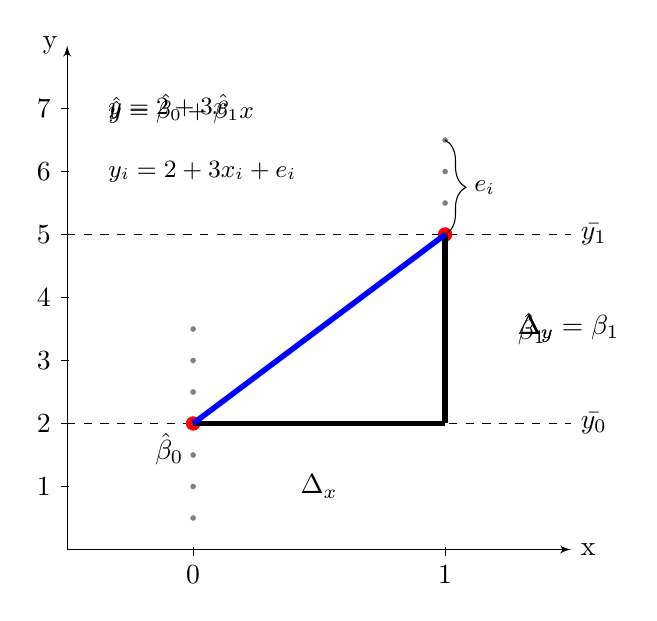
\begin{tikzpicture}[>=latex', scale=0.8]
        \draw[->] (0,0) node[below] (origin) {}  -- (8,0) node[right] (xaxis) {x};
        \draw[->] (origin) -- (0,8) node[left] (yaxis) {y};
        % x ticks
        \draw (2,1pt) -- (2,-3pt) node[anchor=north] {0};
        \draw (6,1pt) -- (6,-3pt) node[anchor=north] {1};
        % y ticks
        \foreach \y in {1,...,7}
             \draw (1pt,\y) -- (-3pt,\y) node[anchor=east] {$\y$};
        
        % points
        \foreach \y in {0.5,1.0,...,3.5} {
        	\draw[gray,fill] (2,\y) circle [radius=1pt];
        	\draw[gray,fill] (6,3+\y) circle [radius=1pt];
        }
        % y_0-bar
        \draw<2-4>[dashed] (0,2) -- (8,2) node[right] {$\bar{y_0}$};
        % y_1-bar
        \draw<2-4>[dashed] (0,5) -- (8,5) node[right] {$\bar{y_1}$};
        % mean points
        \draw<2->[red,fill] (2,2) circle [radius=3pt];
        \draw<2->[red,fill] (6,5) circle [radius=3pt];
        
        % slope
        \draw<3-4>[solid, line width=2pt] (2,2) -- (6,2);
        \draw<3-5>[solid, line width=2pt] (6,2) -- (6,5);
        \node<3-4>(deltax) at (4,1) {$\Delta_x$};
        \node<3>[right](deltay) at (7,3.5) {$\Delta_y$};
        \node<4>[right](deltay) at (7,3.5) {$\Delta_y = \beta_1$};
        \node<5>[right](deltay) at (7,3.5) {$\hat{\beta}_1$};
        
        \draw<4->[blue, solid, line width=2pt] (2,2) -- (6,5);
        \node<4-5>[below left](b0) at (2,2) {$\hat{\beta}_0$};
        
        \node<5>[right](eq) at (0.5,7) {\small $\hat{y} = \hat{\beta}_0 + \hat{\beta}_1 x$};
        \node<6->[right](eq) at (0.5,7) {\small $\hat{y} = 2 + 3 x$};
        \node<7->[right](eq) at (0.5,6) {\small $y_i = 2 + 3 x_i + e_i$};
        \draw<7->[right,decorate,decoration={brace,mirror,amplitude=7.5pt}] (6,5)  -- (6,6.5)
        	node [right, pos=0.5, xshift=7] {\small $e_i$};
    \end{tikzpicture}
    \end{center}
}

% OLS only makes sense in a linear world

\frame{
	\frametitle{Systematic versus unsystematic component of the data}
	\begin{itemize}\itemsep1em
    	\item Systematic: Regression line (slope)
    		\begin{itemize}
    		\item Linear regression fits the conditional mean of the data (i.e., $E[Y|X=x]$)
    		\end{itemize}
    	\item Unsystematic: Error term is the deviation of observations from the line
    		\begin{itemize}
        		\item The difference between each value $Y_i$ and $E[Y|X=X_i]$ is the \textit{residual}: $e_i$
        		\item OLS produces an estimate of the relationship between X and Y that minimizes the \textit{residual sum of squares}
    		\end{itemize}
	\end{itemize}
}

\frame{
	\frametitle{Why are there residuals?}
	\begin{itemize}\itemsep1em
		\item<2-> Omitted variables
		\item<2-> Measurement error
		\item<2-> Fundamental randomness
	\end{itemize}
}

\againframe<2-3>{dummy}

\againframe<2-3>{ways}


\frame{
	\frametitle{Bivariate Regression II}
	\begin{itemize}\itemsep1em
	\item $Y$ is continuous
	\item $X$ is continuous (and randomized)
	\item How do we know if the treatment $X$ had an effect on $Y$?
		\begin{itemize}
		\item Correlation coefficient ($\rho$)
		\item Regression coefficient (slope; $\beta_1$)
		\end{itemize}
	\end{itemize}
}

\frame<1>[label=correlation]{
	\frametitle{Correlation Coefficient ($\rho$)}
	\begin{itemize}\itemsep1em
	\item Measures how well a scatterplot is represented by a straight line
	\item<2-> Formal definition: 
		$\frac{Cov(X,Y)}{\sigma_X \sigma_y}$
	\item<2-> As a reminder:\\
		\begin{itemize}\itemsep1em
		\item $Cov(x,y) = \sum_{i=1}^{n}(x_i - \bar{x})(y_i - \bar{y})$
		\item $s_x = \sqrt{\sum_{i=1}^{n}(x_i - \bar{x})^2}$
		\end{itemize}
	\end{itemize}
}

\frame{
	\includegraphics[width=\textwidth]{images/correlation}
}

\againframe<1->{correlation}

\frame{
	\frametitle{OLS Coefficient ($\beta_1$)\footnote{Multivariate formula involves matrices; Week 20}}
	\begin{itemize}\itemsep1em
	\item Measures $\Delta Y$ given $\Delta X$
	\item<2-> Formal definition: 
		$\frac{Cov(X,Y)}{Var(X)}$
	\item<2-> As a reminder:\\
		\begin{itemize}\itemsep1em
		\item $Cov(x,y) = \sum_{i=1}^{n}(x_i - \bar{x})(y_i - \bar{y})$
		\item $Var(x) = \sum_{i=1}^{n}(x_i - \bar{x})^2$
		\end{itemize}
	\item<3-> $\hat{\rho}$ and $\hat{\beta_1}$ are just scaled versions of $\widehat{Cov}(x,y)$
	\end{itemize}
}

\frame<1-6>[label=math]{
	\frametitle{Minimum Mathematical Requirements}
	\begin{enumerate}\itemsep1em
    	\item<1-> Do we need variation in $X$?
    		\begin{itemize}
        		\item<2-> Yes, otherwise dividing by zero
    		\end{itemize}
    	\item<3-> Do we need variation in $Y$?
    		\begin{itemize}
        		\item No, $\hat{\beta}_1$ can equal zero
    		\end{itemize}
    	\item<5-> How many observations do we need?
    		\begin{itemize}
    		\item<6-> $n \ge k$, where $k$ is number of parameters to be estimated
    		\end{itemize}
    	\item<7-> Can we have highly correlated regressors?
    		\begin{itemize}
    		\item<8-> Generally no.
    		\end{itemize}
	\end{enumerate}
}

\frame<1-5>[label=scatter]{
	\begin{center}
	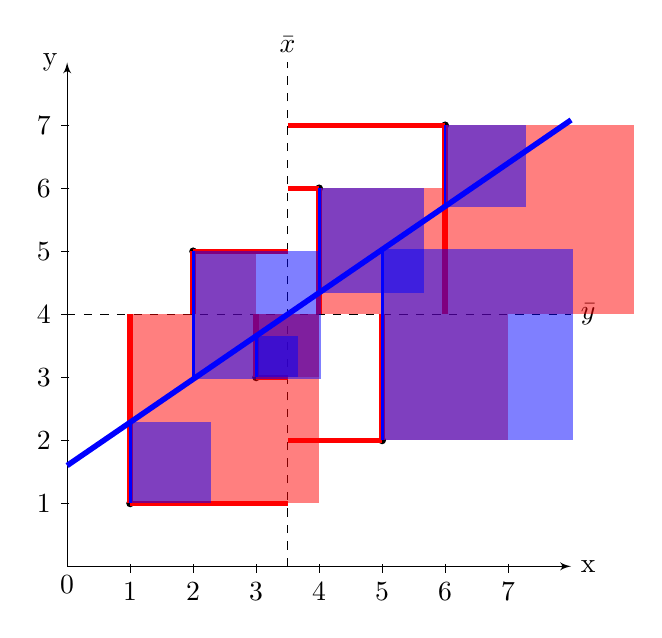
\begin{tikzpicture}[>=latex', scale=0.8]
        \draw[->] (0,0) node[below] (origin) {0}  -- (8,0) node[right] (xaxis) {x};
        \draw[->] (origin) -- (0,8) node[left] (yaxis) {y};
        % x ticks
        \foreach \x in {1,...,7}
        	\draw (\x,1pt) -- (\x,-3pt) node[anchor=north] {$\x$};
        % y ticks
        \foreach \y in {1,...,7}
             \draw (1pt,\y) -- (-3pt,\y) node[anchor=east] {$\y$};
        % points
        \draw[fill] (1,1) circle [radius=1.5pt];
        \draw[fill] (2,5) circle [radius=1.5pt];
        \draw[fill] (3,3) circle [radius=1.5pt];
        \draw[fill] (4,6) circle [radius=1.5pt];
        \draw[fill] (5,2) circle [radius=1.5pt];
        \draw[fill] (6,7) circle [radius=1.5pt];
        % x-bar
        \draw<2->[dashed] (3.5, 0) -- (3.5,8) node[above] {$\bar{x}$};
        % y-bar
        \draw<2->[dashed] (0,4) -- (8,4) node[right] {$\bar{y}$};
        
        % x-deviations
        \draw<3>[red, line width=2pt] (1,1) -- (3.5,1);
        \draw<3>[red, line width=2pt] (2,5) -- (3.5,5);
        \draw<3>[red, line width=2pt] (3,3) -- (3.5,3);
        \draw<3>[red, line width=2pt] (4,6) -- (3.5,6);
        \draw<3>[red, line width=2pt] (5,2) -- (3.5,2);
        \draw<3>[red, line width=2pt] (6,7) -- (3.5,7);
        % y-deviations
        \draw<4,6-7,10-11>[red, line width=2pt] (1,1) -- (1,4);
        \draw<4,6-7,10-11>[red, line width=2pt] (2,5) -- (2,4);
        \draw<4,6-7,10-11>[red, line width=2pt] (3,3) -- (3,4);
        \draw<4,6-7,10-11>[red, line width=2pt] (4,6) -- (4,4);
        \draw<4,6-7,10-11>[red, line width=2pt] (5,2) -- (5,4);
        \draw<4,6-7,10-11>[red, line width=2pt] (6,7) -- (6,4);
        
		\fill<7,11>[red, opacity=0.5] (1,1) rectangle (4,4);
		\fill<7,11>[red, opacity=0.5] (2,5) rectangle (3,4);
		\fill<7,11>[red, opacity=0.5] (3,3) rectangle (4,4);
		\fill<7,11>[red, opacity=0.5] (4,6) rectangle (6,4);
		\fill<7,11>[red, opacity=0.5] (5,2) rectangle (7,4);
		\fill<7,11>[red, opacity=0.5] (6,7) rectangle (9,4);

        % line
        \draw<5->[blue, line width=2pt] (0,1.6) -- (8,7.0856);
        
        % residuals
        \draw<8->[blue, line width=1pt] (1,1) -- (1,2.29);
        \draw<8->[blue, line width=1pt] (2,5) -- (2,2.97);
        \draw<8->[blue, line width=1pt] (3,3) -- (3,3.66);
        \draw<8->[blue, line width=1pt] (4,6) -- (4,4.34);
        \draw<8->[blue, line width=1pt] (5,2) -- (5,5.03);
        \draw<8->[blue, line width=1pt] (6,7) -- (6,5.71);
		
		\fill<9-11>[blue, opacity=0.5] (1,1) rectangle (2.29,2.29);
		\fill<9-11>[blue, opacity=0.5] (2,5) rectangle (4.03,2.97);
		\fill<9-11>[blue, opacity=0.5] (3,3) rectangle (3.66,3.66);
		\fill<9-11>[blue, opacity=0.5] (4,6) rectangle (5.66,4.34);
		\fill<9-11>[blue, opacity=0.5] (5,2) rectangle (8.03,5.03);
		\fill<9-11>[blue, opacity=0.5] (6,7) rectangle (7.29,5.71);

		
    \end{tikzpicture}
    \end{center}
}

\frame{
	\frametitle{Calculations}
	\begin{tabular}{rrrrrr} \hline
	$x_i$ & $y_i$ & $x_i - \bar{x}$ & $y_i - \bar{y}$ & $(x_i - \bar{x})(y_i - \bar{y})$ & $(x_i - \bar{x})^2$\\ \hline
	1 & 1 & ? & ? & ? & ? \\
	2 & 5 & ? & ? & ? & ? \\
	3 & 3 & ? & ? & ? & ? \\
	4 & 6 & ? & ? & ? & ? \\
	5 & 2 & ? & ? & ? & ? \\
	6 & 7 & ? & ? & ? & ? \\ \hline
	\end{tabular}
}
% mean(x) = 3.5
% mean(y) = 4
% cov(x,y) = 12
% var(x) = 17.5
% slope = 0.6857143

\frame{
	\frametitle{Intercept $\hat{\beta}_0$}
	\begin{itemize}\itemsep1em
	\item Simple formula: $\hat{\beta}_0 = \bar{y} - \hat{\beta}_1 \bar{x}$
	\item<2-> Intuition: OLS fit always runs through point $(\bar{x}, \bar{y})$
	\item<3-> Ex.: $\hat{\beta}_0 = 4 - 0.6857 * 3.5 = 1.6$
	\item<4-> $\hat{y} = 1.6 + 0.6857 \hat{x}$
	\end{itemize}
}

\againframe<5>{scatter}

% CEF: compare $\bar{Y}$ and $E[Y|X=x]$

\againframe<3-4>{ways}


\frame{
	\frametitle{OLS Minimizes SSR}
	\begin{itemize}\itemsep1em
    	\item Total Sum of Squares (SST): $\sum_{i=1}^{n}(y_i - \bar{y})^2$
    	\item We can partition SST into two parts (ANOVA):
    		\begin{itemize}
    		\item Explained Sum of Squares (SSE)
    		\item Residual Sum of Squares (SSR)
    		\end{itemize}
    	\item $SST = SSE + SSR$
    	\item OLS is the line with the lowest SSR
	\end{itemize}
}

\againframe<5-11>{scatter}




\frame{
	\frametitle{Are Our Estimates Any Good?}
	\begin{itemize}\itemsep1em
    	\item Yes, if:\\
    		\begin{enumerate}\itemsep1em
        		\item Works mathematically
        		\item Causally valid theory
        		\item Linear relationship between $X$ and $Y$
        		\item $X$ is measured without error
        		\item No missing data
        		\item No confounding
    		\end{enumerate}
    	\item Let's go through these points
	\end{itemize}
}


\frame{
	\frametitle{Aside: Three Meanings of ``Endogeneity''}
	Formally endogeneity is when $Cov(X,\epsilon) \neq 0$
	\vspace{1em}
	\begin{enumerate}\itemsep1em
	\item Measurement error in regressors
	\item Omitted variables associated with included regressors 
		\begin{itemize}
		\item ``Specification error''
		\item Confounding
		\end{itemize}
	\item Lack of temporal precedence
	\end{enumerate}
}


\frame{
	\frametitle{Aside: Squared vs. Absolute Deviations}
	\begin{itemize}\itemsep1em
	\item Conventionally use SSR
	\item Using absolute deviations is also unbiased
	\item SSR has a smaller variance
	\item SSR more heavily weights outliers
	\item Thus OLS is BLUE
	\end{itemize}
}


\frame{
	\frametitle{Linear Relationship}
	\begin{itemize}\itemsep1em
    	\item If linear, no problems
    	\item If non-linear, we need to transform
    		\begin{itemize}
        		\item Power terms (e.g., $x^2$, $x^3$)
        		\item log (e.g., $log(x)$)
        		\item Other transformations
        		\item If categorical: convert to set of indicators
        		\item Multivariate interactions (next week)
    		\end{itemize}
	\end{itemize}
}

\frame{
	\frametitle{Coefficient Interpretation Activity}
	\begin{itemize}\itemsep1em
	\item Four types of variables:
		\begin{enumerate}
		\item Indicator (0,1)
		\item Categorical
		\item Ordinal
		\item Interval
		\end{enumerate}
	\item How do we interpret a coefficient on each of these types of variables?
	\end{itemize}
}

\frame{
	\frametitle{Notes on Interpretation}
	\begin{itemize}\itemsep1em
	\item<1-> Effect $\beta_1$ is constant across values of $x$
	\item<2-> That is not true when there are:
		\begin{itemize}
		\item Interaction terms (next week)
		\item Nonlinear transformations (e.g., $x^2$)
		\item Nonlinear regression models (e.g., logit/probit)
		\end{itemize}
	\item<3-> Interpretations are sample-level
		\begin{itemize}
		\item Sample representativeness determines generalizability
		\end{itemize}
	\item<4-> Remember uncertainty
		\begin{itemize}
		\item These are \textit{estimates}, not population parameters
		\end{itemize}
	\end{itemize}
}



\frame{
	\frametitle{Measurement Error in Regressor(s)}
	\begin{itemize}\itemsep1em
    	\item We want effect of $x$, but we observe $x^{*}$, where $x = x^{*} + w$:
    	\begin{align*}
    	y & = \beta_0 + \beta_1 x^{*} + \epsilon\\
    	y & = \beta_0 + \beta_1 (x - w) + \epsilon\\
    	y & = \beta_0 + \beta_1 x + (\epsilon - \beta_1 w)\\
    	y & = \beta_0 + \beta_1 x + v
    	\end{align*}
	\end{itemize}
}

\frame{
	\frametitle{Measurement Error in Regressor(s)}
	\begin{itemize}\itemsep1em
    	\item Produces \textit{attenuation}: as measurement error increases, $\beta_1 \rightarrow 0$
    	\item Our coefficients fit the observed data
    	\item But they are \textit{biased} estimates of our population equation
    		\begin{itemize}
    		\item This applies to all $\hat{\beta}$ in a multivariate regression
    		\end{itemize}
	\end{itemize}
}


\frame{
	\frametitle{Measurement Error in $Y$}
	\begin{itemize}\itemsep1em
    	\item Not necessarily a problem
    	\item If \textit{random} (i.e., uncorrelated with $x$), it costs us precision
    	\item If \textit{systematic}, who knows?!
    	\item Special case: \textit{censoring} (see Lectures 11 and/or 12)
	\end{itemize}
}


\frame{
	\frametitle{Missing Data}
	\begin{itemize}\itemsep1em
	\item Missing data can be a big problem
	\item We will discuss it in Lecture 5
	\end{itemize}
}

\frame{
	\frametitle{Confounding (Selection Bias)}
	\begin{itemize}\itemsep1em
	\item If $x$ is not randomly assigned, potential outcomes are not independent of $x$
	\item Other factors explain why units received their particular value $x_i$
	\vspace{1em}
	\item In matching, we obtain \textit{conditional independence} by comparing units that are identical on all confounding variables
	\end{itemize}
}

\frame{
	\frametitle{Omitted Variables}
	{\small
	$\underbrace{E[Y_i| X_i = 1] - E[Y_i | X_i = 0] =}_{\text{Naive Effect}}$\\
	\vspace{1em}
	$\underbrace{E[Y_{1i}|X_i =1] - E[Y_{0i} | X_i = 1]}_{\text{Treatment Effect on Treated (ATT)}} + \underbrace{E[Y_{0i}|X_i = 1] - E[Y_{0i}|X_i=0]}_{\text{Selection Bias}}$
	}
	\vspace{1em}
}


\frame{

SHOW BIAS HERE

}

\frame[label=causalgraph]{
	\begin{center}
	\begin{tikzpicture}[>=latex',circ/.style={draw, shape=circle, node distance=5cm, line width=1.5pt}]
        \draw[->] (0,0) node[left] (X) {X} -- (2.5,0) node[right] (D) {D};
        \draw[->] (3.1,0) -- (5,0) node[right] (Y) {Y};
        \draw[->] (-3,4) node[above] (Z) {Z} -- (X);
        \draw[->] (Z) -- (Y);
        \draw[->] (5,2) node[above] (A) {A} -- (Y);
        \draw[->] (-2,0) node[left] (B) {B} -- (X);
        \draw[->] (X) -- (2,-2) node[right] (C) {C};
    \end{tikzpicture}
    \end{center}
}

\frame{
	\frametitle{Example: Englebert}
	\begin{itemize}\itemsep2em
	\item What is his research question?
	\item What is his theory? What does the graph look like?
	\item What is his analysis?
	\end{itemize}
}


\frame{
	\frametitle{Common Conditioning Strategies}
	\begin{enumerate}\itemsep1em
    	\item<2-> Condition on nothing (``naive effect'')
    	\item<3-> Condition on some variables
    	\item<4-> Condition on all observables
	\end{enumerate}
}


\frame<1-3>[label=what]{
	\frametitle{What goes in our regression?}
	\begin{itemize}\itemsep1em
    	\item Use theory to build causal models
    		\begin{itemize}
    		\item Often, a causal graph helps
    		\end{itemize}
    	\item Some guidance:
    		\begin{itemize}
    		\item<2-> Include confounding variables
	    	\item<3-> Do not include post-treatment variables
	    	\item<4-> Do not include \textit{colinear} variables
    		\item<5-> Including irrelevant variables costs certainty
    		\item<6-> Including variables that affect $Y$ alone increases certainty
    		\end{itemize}
	\end{itemize}
}

\againframe{causalgraph}

\frame{
	\frametitle{Post-treatment Bias}
	\begin{itemize}
	\item We usually want to know the \textbf{total effect} of a cause
	\item If we include a mediator, $D$, of the $X \rightarrow Y$ relationship, the coefficient on $X$:
		\begin{itemize}
    		\item Only reflects the \textbf{direct} effect
    		\item Excludes the \textbf{indirect} effect of $X$ through $M$
		\end{itemize}
	\item So don't control for mediators!
	\end{itemize}
}

\againframe<3-4>{what}

\againframe<6-8>{math}

\againframe<4-6>{what}

\againframe{causalgraph}

\frame{
	\frametitle{Multivariate Regression Interpretation}
	\begin{itemize}\itemsep1em
	\item All our interpretation rules from earlier still apply in a multivariate regression
	\item Now we interpret a coefficient as an effect ``all else constant''
	\item Generally, not good to give all coefficients a causal interpretation
		\begin{itemize}
		\item Think ``forward causal inference''
		\item We're interested in the $X \rightarrow Y$
		\item All other coefficients are there as ``controls''
		\end{itemize}
	\end{itemize}
}


\frame{
	\frametitle{OLS is BLUE}
	
	
	
	
}


%OLS is BLUE due to the Gauss-Markov assumptions
%1. Linearity in parameters
%2. Random sampling
%3. No collinearity
%4. Expected value of errors is zero
%5. Homoskedasticity


\section{Goodness-of-Fit}
\frame{\tableofcontents[currentsection]}

\frame{
	\frametitle{Goodness-of-Fit}
	\begin{itemize}\itemsep1em
	\item We want to know: ``How good is our model?''
	\item<2-> We can answer:\\
		``How well does our model fit the observed data?''
	\item<3-> Is this what we want to know?
	\end{itemize}
}

\frame{
	\frametitle{Correlation}
	\begin{itemize}\itemsep1em
	\item Definition: $corr(x,y) = \hat{r}_{x,y} = \frac{cov(x,y)}{(n-1)sd(x)sd(y)}$
	\item Slope $\hat{\beta}_1$ and correlation $\hat{r}_{x,y}$ are simply different scalings of $cov(x,y)$
	\item Interpretation: How well the bivariate relationship is summarized by a cloud of points?
	\item Units: none (range 0 to 1)
	\end{itemize}
}

\frame{
	\frametitle{Coefficient of Determination ($R^2$)}
	\begin{itemize}\itemsep1em
	\item Definition: $R^2 = cor(x,y)^2 = \frac{SSE}{SST} = 1 - \frac{SSR}{SST}$
	\item Interpretation: How much of the total variation in $y$ is explained by the model?
	\item But, $R^2$ increases simply by adding more variables
	\item So, $Adj.R^2 = R^2 - (1 - R^2)\frac{k}{n-k-1}$, where $k$ is number of regressors
	\item Units: none (range 0 to 1)
	\end{itemize}
}

\frame{
	\frametitle{Standard Error of the Regression (SER)}
	\begin{itemize}\itemsep1em
	\item ``Root mean squared error'' or just $\sigma$
	\item Definition: $\hat{\sigma} = \sqrt{\frac{SSR}{n-p}}$, where $p$ is number of parameters estimated
	\item Interpretation: How far, on average, are the observed $y$ values from their corresponding fitted values $\hat{y}$
		\begin{itemize}
		\item $sd(y)$ is how far, on average, a given $y_i$ is from $\bar{y}$
		\item $\sigma$ is how far, on average, a given $y_i$ is from $\hat{y}_i$
		\end{itemize}
	\item Units: same as $y$ (range 0 to $sd(y)$)
	\end{itemize}
}

\frame{
	\frametitle{The F-test}
	\begin{itemize}\itemsep1em
	\item Definition: Test of whether any of our coefficients differ from zero
		\begin{itemize}
		\item In a bivariate regression, $F=t^2$
		\end{itemize}
	\item Interpretation: Do any of the coefficients differ from zero?
		\begin{itemize}
		\item Not a very interesting measure
		\end{itemize}
	\item Units: none (range 0 to $\infty$)
	\end{itemize}
}

\begin{frame}[fragile]
\scriptsize
\begin{verbatim}
. reg growth lcon

      Source |       SS       df       MS              Number of obs =      44
-------------+------------------------------           F(  1,    42) =    0.09
       Model |  .000038348     1  .000038348           Prob > F      =  0.7615
    Residual |  .017255198    42  .000410838           R-squared     =  0.0022
-------------+------------------------------           Adj R-squared = -0.0215
       Total |  .017293546    43  .000402175           Root MSE      =  .02027

------------------------------------------------------------------------------
      growth |      Coef.   Std. Err.      t    P>|t|     [95% Conf. Interval]
-------------+----------------------------------------------------------------
        lcon |  -.0017819   .0058325    -0.31   0.761    -.0135524    .0099886
       _cons |   .0158988   .0390155     0.41   0.686    -.0628376    .0946353
------------------------------------------------------------------------------

\end{verbatim}
\end{frame}

\frame{
	\frametitle{The F-test for nested models}
	\begin{itemize}
	\item Can use an F-test to compare fit of two nested models?
		\begin{itemize}
		\item $\hat{y} = \hat{\beta_0} + \hat{\beta_1}x_1$
		\item $\hat{y} = \hat{\beta_0} + \hat{\beta_1}x_1 + \hat{\beta_2}x_2 + \dots$
		\end{itemize}
	\item \textit{Reduced} model is nested within \textit{expanded} model
	\item Interpretation: Does adding additional variables significantly reduce SSR?
	\end{itemize}
}


\begin{frame}[fragile]
\footnotesize

\begin{verbatim}
. nestreg: reg growth lcon (lconsq)

+-------------------------------------------------------------+
                Block  Residual                     Change 
Block        F     df        df   Pr > F       R2    in R2 
-------+-----------------------------------------------------
1         0.09      1        42   0.7615   0.0022          
2         7.98      1        41   0.0073   0.1649   0.1626 
+-------------------------------------------------------------+

\end{verbatim}
\end{frame}





\section{Inference}
\frame{\tableofcontents[currentsection]}

\frame{
	\frametitle{Inference from Sample to Population}
	\begin{itemize}\itemsep1em
	\item We want to know population parameter $\theta$
	\item We only observe sample estimate $\hat{theta}$
	\item We therefore have a guess, but we are also uncertain
	\vspace{1em}
	\item What range of values for $\theta$ does our $\hat{theta}$ imply?
	\end{itemize}
}





\frame{
	\frametitle{Significance}
	\begin{enumerate}\itemsep2em
    	\item Substantive significance
    		\begin{itemize}
        		\item<2-> Is the effect size \textit{important} in the real world?
    		\end{itemize}
    	\item Statistical significance
    		\begin{itemize}
        		\item<3-> Is the effect size larger than a predetermined threshold?
    		\end{itemize}
	\end{enumerate}
}




\begin{comment}




% To draw inferences about the population, we need to account for uncertainty in our estimates
% We do this by generating standard errors (SEs) for the regression estimates

% SEs
	% Definition: The standard error of a sample estimate is the average distance that a sample estimate would be from the population value if we drew lots and lots of separate random samples.
	% If we repeated our sampling procedure an infinite number of times, the SE is the average deviation of a sample estimate from the population mean
	% Standard errors are based on assumptions about the sampling process, not anything about our sample data per se
	
	
SE Interpretation

  - SE is a ratio of unexplained variance in `\(y\)` (weighted by sample size) and variance in `\(x\)`

  - More variance in `\(x\)` means smaller SE

  - More unexplained variance in `\(y\)` means bigger SE

  - More observations yields smaller numerator in `\(s_{\hat{\beta_1}}\)`, meaning smaller SE

  - The SE has the units of the coefficient (i.e., `\(y\)` per `\(x\)`))
  
  $var(\hat{\beta_1}) = \frac{\frac{1}{n-2}RSS}{SS_x}$
  $s_{\hat{\beta_1}} = \sqrt{\frac{\frac{1}{n-2}RSS}{SS_x}} = \sqrt{\frac{\sigma^2}{SS_x}}$
  % more complicated in a multivariate regression
  
  
## Homoskedasticity and heteroskedasticity

  - The basic SE formula (and the default calculations in Stata) assume homoskedasticity
  
  - When errors are heteroskedastic, we need ``robust'' SEs

  - David will cover this in Lecture 4

% assumption of Normality
% $y|x \sim N(\beta_0 + \beta_1x_1 + ..., \sigma^2)$
% There is a population of identically distributed cases of which our data are one sample

% t-statistics
% regression on population versus sample versus super-population
% The sampling distribution for `\(\beta_1\)` that we just assumed (partially based on our data), allows us to conduct hypothesis tests
% The kinds of hypotheses we can test are of the form:
	% Bivariate: ``$X$ has no effect on $Y$''
	% Multivariate: ``accounting for the other variables in the model, $X$ has no effect on the expected value of $Y$''

% often use a no-effect null hypothesis, but we can do anything
% $\frac{\hat{\beta_1} - \alpha}{SE_{\hat{\beta_1}}}$, where $\alpha$ is our null hypothesis value

% - The $t$*-statistic from a $t$-test of mean-difference is the same as the $t$-statistic from a $t$-test on an OLS slope for a dummy covariate
% $t_{\hat{\beta_1}} = \frac{\hat{\beta_1}}{SE_{\hat{\beta_1}}}$
% we then go back to the $t$-distribution function (which tells us how likely a given $t$-ratio is)

% The p-value is the probability of seeing a t-ratio/t-statistic as large or larger than the one we observed in our data

Definition of p-value:

the probability of a *t*-statistic as extreme as the one we observed, if the null hypothesis was true

the probability of a slope as large as the one we observed, given the observed variance in the data and that the null hypothesis was true


The p-value is not:

  - The probability that a hypothesis is true or false

  - A reflection of our confidence or certainty about the result

  - The probability that the true slope is in any particular range of values

  - A statement about the importance or substantive size of the effect
  
  
A CI is simply a range, centered on the slope
CIs and p-values convey the same information
CIs are on the scale of the statistic of interest (and thus the scale of the original data)
If the confidence interval overlaps zero, we would be unable to reject the null the hypothesis

Definition: Were we to repeat our procedure of sampling, analyzing the sample, and calculating a confidence interval *repeatedly* from the population, a fixed percentage of the resulting intervals would include the true population-level slope.

We cannot say for sure whether the estimated confidence interval *this time* actually includes that true slope



\end{comment}



\appendix
\frame{}

\end{document}
